%
% File ACL2016.tex
%

\documentclass[11pt]{article}
\usepackage{acl2016}
\usepackage{times}
\usepackage{url}
\usepackage{latexsym}

%███████████████████ USER PACKAGES ███████████████████
%%\usepackage{etex}
\usepackage{tikz-qtree-compat}	% draw trees with simple syntax
\usepackage{forest}
\usepackage{amsmath}
\usepackage{amsfonts}	% e.g. \leadsto symbol
%\usepackage{bm}
%%\usepackage{amssymb}
%%\usepackage{calc}
%%\usepackage{caption} 	% several captions and subfloats
%\usepackage[labelfont=bf, labelsep=period]{caption} % formatting caption
%\usepackage[labelfont=normalfont]{subcaption} % subcaptions for subfloats
%%\usepackage{enumerate}
%\usepackage[printwatermark]{xwatermark} % forwatermarks
\usepackage{enumitem}	% enumerating with referencing
%\usepackage{cite}     	% allows [1,2] reference style 
%\usepackage{authordate1-4}
%%\usepackage{graphicx}
%\usepackage[table]{xcolor} % color tabular clashes with hyperref 
\usepackage{colortbl} 		% colored tabular
\usepackage[normalem]{ulem}
%\bibliographystyle{authordate1}	
%\usepackage[colorlinks=true, linkcolor=black, citecolor=black, urlcolor=black, breaklinks]{hyperref}	% referencing enhancement
%%\usepackage{tikz}
%%\usetikzlibrary{arrows,automata} % draw automata
%%\usetikzlibrary{shapes, positioning}  % snakes
%%\usepackage{bussproofs}
%%\usepackage{array}
%%\usepackage{linguex}
%%\usepackage{cgloss4e}
%%\usepackage{mathalfa}
%%\usepackage{mathtools}
\usepackage[e]{esvect}  	% vector sign above a symbol
%%\usepackage{bm}
%%\usepackage[titletoc,toc,title]{appendix}
\usepackage{slashbox} 		% diagonal in the table cell
\usepackage{multirow}		% cell spanning in tabular
%\usepackage[noabbrev]{cleveref}
%\usepackage[bottom]{footmisc} %will insert additional whitespace between the main text and the footnote rule rather than over-stretching the inter-paragraph glue
%\usepackage{euler}
%\usepackage{qtree}
% \makebox[\textwidth][c]{}
%\usepackage{todonotes} 		% to add notes
\usepackage{tcolorbox}		% for labels of the nodes
\usepackage{todonotes} % to add notes

\usetikzlibrary{backgrounds}


%████████████ USER DEFINED COMMANDS ████████████

\newcommand{\candc}{C\&C}
\newcommand{\easyccg}{EasyCCG}
\newcommand{\ccg}{\textsc{ccg}}
\newcommand{\sick}{SICK}
\newcommand{\fracas}{{\sc f}ra{\sc c}a{\sc s}}
%\newcommand{\langpro}{{\sc l}ang{\sc p}ro}
\newcommand{\langpro}{LangPro}
\newcommand{\llfgen}{LLFgen}
%\newcommand{\llfaligner}{LLFaligner}
\newcommand{\pofs}{{\sc pos}}
\newcommand{\nlogpro}{NLogPro}
\newcommand{\gold}{\textsc{gold}}
\newcommand{\ent}{${\tt entailment}$}
\newcommand{\cont}{${\tt contradiction}$}
\newcommand{\neut}{${\tt neutral}$}
\newcommand{\mytep}{\textsc{tep}}
\newcommand{\elist}{\scalebox{.9}{[\kern1pt]}}
\newcommand{\clrule}{$\leq\!$\raisebox{-1pt}{\scalebox{1.4}{$\times$}}}
\newcommand{\btimes}{\scalebox{1.15}{$\times$}\kern-1.5pt}
\newcommand{\rulen}[1]{{\normalfont\textsc{#1}}}
\newcommand{\ruleApp}[2][]{\textsc{#2}[#1]}
\newtcbox{\lab}[1][white]{on line, arc=1.5pt, colframe=black!30, colback=#1, %before upper={\rule[-3pt]{0pt}{10pt}}, 
	boxrule=.5pt, boxsep=0pt, left=1pt, right=1pt, top=1pt, bottom=1pt}
\newcommand{\toppad}[1]{\rule{0pt}{#1}}
\newcommand{\botpad}[1]{\rule[#1]{0pt}{0pt}}
\newcommand{\push}{\scalebox{.75}[1]{$>$}}
\newcommand{\pull}{\scalebox{.75}[1]{$<$}}

\newcommand{\comments}[1]{}
\newcommand{\addlater}[1]{\todo[line,size=\tiny]{#1}}
\newcommand{\semt}[1]{\tt #1}
\newcommand{\synt}[1]{\textbf{#1}}
\newcommand{\sem}[1]{[\![#1]\!]}


\newcommand{\X}{\mathbb{X}}
\newcommand{\T}{\mathbb{T}}
\newcommand{\F}{\mathbb{F}}
% \To
\newcommand{\To}{\!\to\!}
\newcommand{\Leq}{\!\leq\!}
\newcommand{\In}{\!\in\!}
\newcommand{\Co}{\!:\!}
\newcommand{\Times}{\!\times\!}
\newcommand{\Pair}[1]{\langle #1 \rangle}
\newcommand{\SetR}[1]{\{ #1 \}}
\newcommand{\SetEl}[1]{\scriptstyle \{ #1 \}}
\newcommand{\MP}{M\!P}
\newcommand{\BS}{\backslash}
\newcommand{\ovA}[1]{\overline{#1\raisebox{7pt}{}}}

%██████████ Categories & Types ██████████
\newcommand{\VP}{{V\!P}}
\newcommand{\NP}{{N\!P}}
\newcommand{\PP}{{P\!P}}
\newcommand{\PR}{P\!R}
\newcommand{\pp}{{\tt pp}}
\newcommand{\np}{{\tt np}}
\newcommand{\sen}{{\tt s}}
\newcommand{\vp}{{\tt vp}}
\newcommand{\nou}{{\tt n}}
\newcommand{\enp}{{e\!n\!p}}

\newcommand{\tabcl}{\times}
\newcommand{\qu}{{\tt q}}
\newcommand{\finval}[1]{(-,#1)}
\newcommand{\lgray}{gray!30}
\newcommand{\grcl}{\cellcolor{gray!25}}

\newcommand{\rd}[1]{\textcolor[rgb]{.65,0,0}{#1}}
\newcommand{\bt}[1]{\textcolor[rgb]{0,0,.65}{#1}}
\newcommand{\gt}[1]{\textcolor[rgb]{0,.5,0}{#1}}


%██████████ Tabulars ██████████
%\newcommand{\tabu}[2][c]{\begin{tabular}{#1}#2\end{tabular}}
\newcommand{\tabuc}[2][t]{\begin{tabular}[#1]{@{}c@{}}#2\end{tabular}}  
\newcommand{\tabur}[2][t]{\begin{tabular}[#1]{@{}r@{}}#2\end{tabular}} 
\newcommand{\tabul}[2][t]{\begin{tabular}[#1]{@{}l@{}}#2\end{tabular}}   

%███ Non Branching Tableau rules
\newcommand{\nonBranchingRule}[3][]{
\begin{tabular}{@{}c@{}}
$\dfrac{
	\begin{tabular}{@{}r@{}}
			#2
	\end{tabular}}
{
	\raisebox{-4pt}{
		\begin{tabular}[t]{@{}r@{}}
   			#3
	\end{tabular}}
}$#1
\end{tabular}}

%███ Branching Tableau rules
\newcommand{\BranchingRule}[4][]{
\begin{tabular}{@{}c@{}}
$\dfrac{  
	\begin{tabular}{@{}r@{}}
			#2
	\end{tabular}
}
{
	\raisebox{-4pt}{
		\begin{tabular}[t]{@{}r@{}}
   			#3
		\end{tabular}} \kern3mm
	\raisebox{-4pt}{
		\begin{tabular}[t]{@{}r@{}}
   			#4
		\end{tabular}}
}$#1
\end{tabular}}

% defining labeltext counter
\newcounter{mylabelcounter}
\makeatletter
\newcommand{\labelText}[2]{%
#1\refstepcounter{mylabelcounter}
\immediate\write\@auxout{%
  \string\newlabel{#2}{{1}{\thepage}{{\unexpanded{#1}}}{mylabelcounter.\number\value{mylabelcounter}}{}}
}%
}
\makeatother

          
%██████████ ACL commands ██████████               
\aclfinalcopy % Uncomment this line for the final submission
%\def\aclpaperid{***} %  Enter the acl Paper ID here

%\setlength\titlebox{5cm}
% You can expand the titlebox if you need extra space
% to show all the authors. Please do not make the titlebox
% smaller than 5cm (the original size); we will check this
% in the camera-ready version and ask you to change it back.

\newcommand\BibTeX{B{\sc ib}\TeX}


\title{Natural Solution to FraCaS Entailment Problems}

% Author information can be set in various styles:
% For several authors from the same institution:
% \author{Author 1 \and ... \and Author n \\
%         Address line \\ ... \\ Address line}
% if the names do not fit well on one line use
%         Author 1 \\ {\bf Author 2} \\ ... \\ {\bf Author n} \\
% For authors from different institutions:
% \author{Author 1 \\ Address line \\  ... \\ Address line
%         \And  ... \And
%         Author n \\ Address line \\ ... \\ Address line}
% To start a seperate ``row'' of authors use \AND, as in
% \author{Author 1 \\ Address line \\  ... \\ Address line
%         \AND
%         Author 2 \\ Address line \\ ... \\ Address line \And
%         Author 3 \\ Address line \\ ... \\ Address line}
% If the title and author information does not fit in the area allocated,
% place \setlength\titlebox{<new height>} right after
% at the top, where <new height> can be something larger than 2.25in

%\author{Lasha  \\
%  Affiliation / Address line 1 \\
%  Affiliation / Address line 2 \\
%  Affiliation / Address line 3 \\
%  {\tt email@domain} \\\And
%  Second Author \\
%  Affiliation / Address line 1 \\
%  Affiliation / Address line 2 \\
%  Affiliation / Address line 3 \\
%  {\tt email@domain} \\}
%
%\date{}

\author{Lasha Abzianidze \\
  TiLPS, Tilburg University, the Netherlands \\
  {\tt L.Abzianidze@uvt.nl}}
\date{}



%████████████████████████ BEGIN ████████████████████████
\begin{document}

\maketitle


%███████████████████ ABSTRACT ██████████████████
\begin{abstract}
Reasoning over several premises is not a common feature of RTE systems as it usually requires deep semantic analysis.
On the other hand, FraCaS is a collection of entailment problems consisting of multiple premises and covering semantically challenging phenomena.
We employ the tableau theorem prover for natural language to solve the FraCaS problems in a {\em natural} way.
The expressiveness of a type theory, the transparency of natural logic and the schematic nature of tableau inference rules make it easy to model challenging semantic phenomena.  
The efficiency of theorem proving also becomes challenging when reasoning over several premises.
After adapting to the dataset, the prover demonstrates state-of-the-art competence over certain sections of FraCaS. 
\end{abstract}

%██████████████████ INTRO ██████████████████
\section{Introduction}

Understanding and automatically processing the natural language semantics is a central task for computational linguistics and its related fields. 
At the same time, inference tasks are regarded as the best way of testing an NLP systems's semantic capacity \cite[p. 63]{fracas}.
Following this view, recognizing textual entailment (RTE) challenges \cite{Dagan:2005} were regularly held which evaluate the RTE systems based on the RTE dataset.
The RTE data represents a set of text-hypotheses pairs that are human annotated on the inference relations: {\em entailment}, {\em contradiction} and {\em neutral}.
Hence it attempts to evaluate the systems on human reasoning.
In general, the RTE datasets are created semi-automatically and are often motivated by the scenarios found in the applications like question answering, relation extraction, information retrieval and summarization \cite{Dagan:2005,rteBook:2013}.
On the other hand, the semanticists are busy designing theories that account for the valid logical relations over natural language sentences.
These theories usually model reasoning that depends on certain semantic phenomena, e.g., Booleans, quantifiers, events, attitudes, intensionality, monotonicity, etc.
These types of reasoning are weak points of RTE systems as the above mentioned semantic phenomena are underrepresented in the RTE datasets. 

%\addlater{We believe that the reason why the RTE problems contain only a single premise is more due to systems' inability to combine properly semantics of several premises than due to high costs of preparing extensive RTE data consisting of multi-premised problems}      

In order to test and train the weak points of an RTE system, we choose the FraCaS dataset \cite{fracas}.
The set contains complex entailment problems covering various challenging semantic phenomena which are still not fully mastered by RTE systems.
Moreover, unlike the standard RTE datasets, FraCaS also allows multi-premised problems. 
To account for these complex entailment problems, we employ the theorem prover for higher-order logic \cite{abzianidze:2015:EMNLP}, which represents the version of formal logic motivated by  {\em natural logic} \cite{lakoff:70,essays:86}. 
Though such expressive logics usually come with the inefficient decision procedures, the prover maintains efficiency by using the inference rules that are specially tailored for the reasoning in natural language.
We introduce new rules for the prover in light of the FraCaS problems and test the rules against the relevant portion of the set.
The test results are compared to the current state-of-the-art on the dataset.
%The experiments also hint that FraCaS does not contain much positive entailments that require higher-order reasoning. 

The rest of the paper is structured as follows. 
We start with introducing a tableau system for natural logic \cite{muskens:10}.
Section~\ref{sec:fracas} explores the FraCaS dataset in more details.
In Section~\ref{sec:model}, we describe the process of adapting the theorem prover to FraCaS, i.e. how specific semantic phenomena are modeled with the help of tableau rules.
%While doing so, we discuss the new rules that account for new semantic phenomena or 
Several premises with monotone quantifiers increase the search space for proofs.
In Section~\ref{sec:efficient}, we present several rules that contribute to shorter proofs.  
In the evaluation part (Section~\ref{sec:eval}), we analyze the results of the prover on the relevant FraCaS sections and compare them with the related RTE systems. 
We end with possible directions of future work.




\begin{figure}[t]
\hspace{-10mm}
\scalebox{.8}{
\begin{forest}
for tree={	align=center, 
			parent anchor=south, 
			child anchor=north, 
			l sep=9mm,
			s sep=0mm}
[{\lab{1}~$\synt{every\,prover}\,(\synt{quickly\,halt}) : \elist : \T$}
 \\{\lab{2}~$\synt{most}\,(\synt{tableau\,prover})\,\synt{terminate} : \elist : \F$}\toppad{5mm}, baseline, node options={label={[label distance=5pt, font=\footnotesize]-90:\ruleApp[1,2]{mon$\uparrow$}}}
 [{\lab{3}~$\synt{quickly\,halt} : [c] : \T$} 
  \\{\lab{4}~$\synt{terminate} : [c] : \F$}\toppad{5mm}
  [{\lab{7}~$\synt{halt} : [c] : \T$}, edge label={node[left,midway,font=\footnotesize]{\ruleApp[3]{$\subseteq$}}}
   [{\lab{15}~$\btimes$}, edge label={node[left,midway,font=\footnotesize]{\ruleApp[4,7]{\clrule}}}
   ] 	
  ] 
 ]
 [{\lab{5}~$\synt{every\,prover} : [P] : \T$} 
  \\{\lab{6}~$\synt{most}\,(\synt{tableau\,prover}) : [P] : \F$}\toppad{5mm}, node options={label={[label distance=7pt, font=\footnotesize]-90:\ruleApp[5,6]{mon$\downarrow$}}}
  [{\lab{8}~$\synt{prover} : [d] : \F$}
   \\{\lab{9}~$\synt{tableau\,prover} : [d] : \T$}\toppad{5mm}
   [{\lab{13}~$\synt{prover} : [d] : \T$}, edge label={node[left,midway,font=\footnotesize]{\ruleApp[9]{$\subseteq$}}}
    [{\lab{14}~$\btimes$}, edge label={node[left,midway,font=\footnotesize]{\ruleApp[8,13]{\clrule}}}
    ]
   ]  	
  ]	
  [{\lab{10}~$\synt{every} : [Q,P] : \T$}
   \\{\lab{11}~$\synt{most} : [Q,P] : \F$}\toppad{5mm}
   [{\lab{12}~$\btimes$}, edge label={node[left,midway,font=\footnotesize]{\ruleApp[10,11]{\clrule}}}
   ] 	
  ]  
 ]
]
\end{forest}
}
\caption{A closed tableau proves that {\em every prover halts quickly} entails {\em most tableau provers terminate}.
Each branch growth is marked with the corresponding rule application.}
\label{fig:intro_proof}
\end{figure}


%██████████████████ Theorem prover ██████████████ 
\section{Tableau theorem prover for natural language}
\label{sec:tableau}

Reasoning in formal logics (i.e., a formal language with well-defined semantics) is carried out by automated theorem provers, where the provers come in different forms based on their underlying proof system.
In order to mirror this scenario for reasoning in natural language, \newcite{muskens:10} proposed to approximate natural language with a version of natural logic \cite{lakoff:70,essays:86,valencia91categorial} while a version of analytic tableau method \cite{beth:55,Hintikka:55,smullyan:1968}, hereafter referred to as {\em natural tableau}, is introduced as a proof system for the logic.
The version of natural logic employed by \newcite{muskens:10} is higher-order logic formulated in terms of the typed lambda calculus \cite{church:1940}.%
%
\footnote{More specifically, the logic is two-sorted variant of Russell's type theory, which according to \newcite{Gallin:1975} represents a more general and neat formulation of \newcite{Montague:1970:EFL}'s intensional logic.
For theorem proving, we employ one-sorted type theory, i.e. with the entity $e$ and truth $t$ types, and hence omit a type $s$ for world-time pairs. 
} 
As a result, the logic is much more expressive (in the sence of modeling certian phenomena in an intuitive way) than first-order logic, e.g., it can naturally account for generalized quantifiers \cite{montague73:PTQ,BarwiseCooper:81}, monotonicity calculus \cite{essays:86,valencia91categorial,icardiMoss:14} and subsective adjectives.


What makes the logic {\em natural} are its terms, called Lambda Logical Forms (LLFs), which are built up only from variables and lexical constants via the functional application and $\lambda$-abstraction.
In this way the LLFs have a more natural appearance than, for instance, the formulas of first-order logic.
The examples of LLFs are given in the nodes of the tableau proof tree in Figure\,\ref{fig:intro_proof}, where the type information for terms is omitted.
A tableau node can be seen as a statement of truth type which is structured as a triplet of a main LLF, an argument list of terms and a truth sign.
The semantics associated with a tableau node is that the application of the main LLF to the terms of an argument list is evaluated according to the truth sign.
For instance, the node \lab{9} is interpreted as the term $\synt{tableau}~\synt{prover}~d$ being true, i.e. $d$ is in the extension of $\synt{tableau}~\synt{prover}$. 
Notice that LLFs not only resemble surface forms in terms of lexical elements but most of their constituents are in correspondence too.
This facilitates the automatized generation of LLFs from surface forms.


\begin{figure}[t]
\centering
\scalebox{.9}{
\tabuc{
\BranchingRule[\rulen{mon$\uparrow$}\\\toppad{5mm}$G$ or $H$ is mon$\uparrow$ and $\vv{d}$ and $P$ are fresh]
{$G~A  : [\vv{C}] : \T$
\\$H~B : [\vv{C}] : \F$}
{$A  : [\vv{d}] : \T$
\\$B : [\vv{d}] : \F$}
{$G  : [P,\vv{C}] : \T$
\\$H : [P,\vv{C}] : \F$}
\\
\\
\BranchingRule[\rulen{mon$\downarrow$}\\\toppad{5mm}$G$ or $H$ is mon$\downarrow$ and $\vv{d}$ and $P$ are fresh]
{$G~A  : [\vv{C}] : \T$
\\$H~B : [\vv{C}] : \F$}
{$A  : [\vv{d}] : \F$
\\$B : [\vv{d}] : \T$}
{$G  : [P,\vv{C}] : \T$
\\$H : [P,\vv{C}] : \F$}
\\
\\
\nonBranchingRule[$\subseteq$ where $A$ is subsective]
{$A~N : [\vv{C}] : \T$}
{$N   : [\vv{C}] : \T$}
\\
\\
\nonBranchingRule[\clrule \parbox{3cm}{where $A$ entails $B$\\written as $A \leq B$}]
{$A : [\vv{C}] : \T$
\\$B: [\vv{C}] : \F$}
{$\btimes$}
}}
\caption{The tableau rules employed by the tableau proof in Figure~\ref{fig:intro_proof}}
\label{fig:intro_rules}
\end{figure} 

The natural tableau system of \cite{muskens:10}, like any other tableau systems \cite{tableauhandbook:99}, tries to prove statements by refuting them.
For instance, in case of an entailment proof, a tableau starts with the counterexample where the premises are true and the conclusion is false.
The proof is further developed with the help of schematic inference rules, called tableau rules (see Figure~\ref{fig:intro_rules}).
A tableau is closed if all its branches are closed, i.e. are marked with a closure ($\!\btimes$) sign.
A tableau branch intuitively corresponds to a situation while a closed branch represents an inconsistent situation.
Refutation of a statement fails if a closed tableau is obtained.
Hence the closed tableau serves as a proof for the statement.    
The proof of an entailment in terms of the closed tableau is demonstrated in Figure~\ref{fig:intro_proof}.
The tableau starts with the counterexample (\lab{1},\lab{2}) of the entailment.
It is further developed by applying the rule (\textsc{mon}$\uparrow$) to \lab{1} and \lab{2}, taking into account that $\synt{every}$ is upward monotone in the second argument position.
The rule application is carried out until all branches are closed or no new rule application is possible.
In the running example, all the branches close as (\clrule) identifies inconsistencies there;
for instance, \lab{4} and \lab{7} are inconsistent according to (\clrule)  assuming that a knowledge base (KB) provides that {\em halting} entails {\em termination}, i.e. $\synt{halt} \leq \synt{terminate}$. 


%On the first view it might seem that the application of \newcite{muskens:10}'s natural tableau system to the natural reasoning is not feasible as building an efficient theorem prover for higher-order logic is extremely challenging.  


The natural tableau system was succesfully applied to the \sick{} textual entailment problems \cite{sick:14} by \newcite{abzianidze:2015:EMNLP}.
In particular, the theorem prover for natural language, called \langpro{}, was implemented that integrates three modules: the parsers for Combinatory Categorial Grammar (CCG) \cite{Steedman:2000}, \llfgen{} that generates LLFs from the CCG derivation trees, and the natural logic tableau prover (\nlogpro{}) which builds tableau proofs.
The pipeline architecture of the prover is depicted in Figure\,\ref{fig:architecture}: the sentences of an input problem are first parsed, then converted into LLFs, which are further processed by \nlogpro{}. 
For a CCG parser, there are at least two options, \candc{} \cite{cc:2007,HonnibalCurranBos2010} and \easyccg{} \cite{lewis-steedman:14}.
The inventory of rules (IR) of \nlogpro{} is a crucial component for the prover; 
it contains most of the rules found in \cite{muskens:10} and also additional rules that were collected from \sick{}.
In order to make theorem proving robust, LangPro employs a conservative extension of the type theory for accessing the syntactic information of terms \cite{abzianidze:2015:LENLS}: in addition to the basic semantic types $e$ and $t$, the extended type theory incorporates basic syntactic types $\nou, \np, \sen$ and $\pp$ corresponding to the primitive categories of CCG.    

\newcite{abzianidze:2015:EMNLP} shows that on the unseen portion of \sick{} LangPro obtains the results comparable to the state-of-the-art scores while achieving an almost perfect precision. 
Based on this inspiring result, we decide to adapt and test LangPro on the FraCaS problems, from the semantics point of view much more harder than the \sick{} ones.%
%
\footnote{An online version of LangPro is available at: \url{http://lanthanum.uvt.nl/labziani/tableau/}
} 



\begin{figure}[t]
\hspace{-3mm}
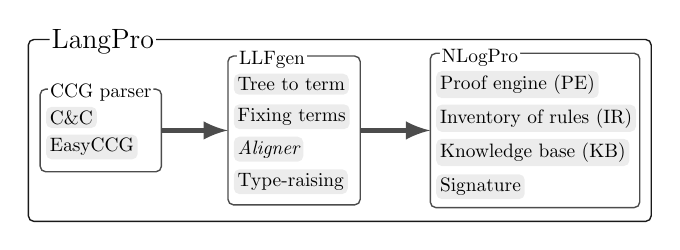
\begin{tikzpicture}[scale=.75]
\def\bgcol{gray!15}
\def\linecol{black!70}

\tikzset{every path/.style={line width=2pt}}
\tikzset{every node/.style={scale=.7, align=center, rounded corners=2pt, rectangle, draw=none, line width=.5pt, inner sep=2pt, outer sep=0pt}}
%\tikzset{node distance=.6cm}
%%%%%%
\node(langpro)at(0,0)[draw=black!90,minimum height=33mm, minimum width=113mm, label={[fill=white,inner sep=1pt,shift={(-4.3,-.3)}]90:{\Large LangPro}}]{};

%%%%%%% CCG parser
\node(parser)at($(langpro.west)+(.2,0)$)[draw=\linecol,anchor=west,minimum height=15mm,minimum width=22mm, label={[inner sep=1pt,fill=white,shift={(0,-.25)}]90:{CCG parser}}]{}; 
\node(cc)at($(parser.north west)+(.1,-.3)$)[fill=\bgcol,anchor=north west]{\candc{}};
\node(easy)at($(cc.west)+(0,-.5)$)[fill=\bgcol,anchor=west]{\easyccg{}};

%%%%%%% LLFgen
\node(llfgen)at($(parser.west)+(4.3,0)$)[draw=\linecol,minimum height=27mm,minimum width=24mm, label={[inner sep=1pt,fill=white,shift={(-.4,-.25)}]90:{\llfgen{}}}]{};
\node(term)at($(llfgen.north west)+(.1,-.3)$)[fill=\bgcol,anchor=north west]{Tree to term};
\node(fix)at($(term.west)+(0,-.55)$)[fill=\bgcol,anchor=west]{Fixing terms};
\node(aligner)at($(fix.west)+(0,-.55)$)[fill=\bgcol,densely dashed,anchor=west]{\em Aligner};
\node(typeraise)at($(aligner.west)+(0,-.55)$)[fill=\bgcol,anchor=west]{Type-raising};

%%%%%%% NatPro
\node(natpro)at($(llfgen.west)+(5.2,0)$)[draw=\linecol,minimum height=28mm,minimum width=38mm, label={[inner sep=1pt,fill=white,shift={(-1,-.27)}]90:{\nlogpro{}}}]{};
\node(pe)at($(natpro.north west)+(.1,-.3)$)[fill=\bgcol,anchor=north west]{Proof engine (PE)};
\node(ir)at($(pe.west)+(0,-.57)$)[fill=\bgcol,anchor=west]{Inventory of rules (IR)};
\node(kb)at($(ir.west)+(0,-.58)$)[fill=\bgcol,anchor=west]{Knowledge base (KB)}; 
\node(sig)at($(kb.west)+(0,-.58)$)[fill=\bgcol,anchor=west]{Signature}; 
%%%%%%%
\path [->,>=latex] (parser.east) edge[draw=\linecol] (llfgen.west);  
\path [->,>=latex] (llfgen.east) edge[draw=\linecol] (natpro.west); 
\end{tikzpicture}
\caption[]{The architecture of LangPro}
\label{fig:architecture} 
\end{figure}      








%██████████████ Fracas ██████████████
\section{FraCaS dataset}
\label{sec:fracas}

The FraCaS test suite \cite{fracas} is a set of 346 test problems.
It was prepared by the FraCaS consortium as an initial benchmark for semantic competence of NLP systems. 
Each FraCaS problem is a pair of premises and a yes-no-unknown question that is annotated with a gold judgment:  {\em yes} (entailment), {\em no} (contradiction), or {\em unknown} (neutral). 
The problems mainly consist of short sentences and resemble the problems found in introductory logic books. 
To convert the test suite into the style of RTE dataset, \newcite{MacCartney:07} translated the questions into declarative sentences.
The judgments were copied from the original test suite with slight modifications.%
%
\footnote{\label{fn:8.7}More details about the conversion, including information about several {\em noisy} problems (e.g., a problem missing a premise or hypothesis, or having a non-standard gold answer) can be found in \newcite{maccartneythesis}.
The FraCaS RTE dataset is available at: \url{http://www-nlp.stanford.edu/~wcmac/downloads/fracas.xml}
}
Several problems drawn from the obtained FraCaS dataset are presented in Table~\ref{tab:problems}.


Unlike other RTE datasets, the FraCaS problems contain multiple premises (45\% of the total problems) and are structured in sections  according to the semantic phenomena they concern. %\addlater{Noisy problems are removed}
The sections cover generalized quantifiers (GQs), plurals, anaphora, ellipsis, adjectives, comparatives, temporal reference, verbs and attitudes.
Due to the challenging problems it contains, the FraCaS dataset can be seen as one of the most complex RTE data from the semantics perspective.
Unfortunately, due to its small size 
%(e.g., some sections have less than 20 problems inside) 
the dataset is not representative enough for system evaluation purposes.   
The above mentioned facts perhaps are the main reasons why the FraCaS data is less favored for developing and assessing the semantic competence of RTE systems.
Nevertheless, several RTE systems \cite{MacCartney:08,naturalli,lewis-steedman:13,tian-miyao-matsuzaki:2014:P14-1,mineshima-EtAl:2015:EMNLP} were trained and evaluated on (the parts of) the dataset.
Usually the goal of these evaluations is to show that specific theories/frameworks and the corresponding RTE systems are able to model deep semantic reasoning over the phenomena found in FraCaS.  
Our aim is also the same in the rest of the sections.
%We adapt  --- to model semantic phenomena also to test the natural tableau system 
%FraCaS is quite small and noisy (see Footnote\,\ref{fn:8.7}) and therefore not a reliable benchmark for comparing RTE systems, but it can be very useful for further development of an RTE system.
%We do so and adapt LangPro to FraCaS.


\begin{table}[t]
\hspace*{-3mm}
\scalebox{.82}{
\begin{tabular}{@{}c@{\kern1pt}|l@{}}\hline
ID  & \hspace{10mm} FraCaS entailment problem
\\\hline%--------------------------------------------
\tabuc[t]{6\\no} & 
\toppad{4mm}\parbox[t]{88mm}{
{\bf P}: No really great tenors are modest.\\
{\bf C}: There are really great tenors who are modest.
}\\\hline%--------------------------------------------
\tabuc[t]{26\\yes} & 
\toppad{4mm}\parbox[t]{88mm}{
{\bf P1}: Most Europeans are resident in Europe.\\
{\bf P2}: All Europeans are people.\\
{\bf P3}: All people who are resident in Europe can travel freely within Europe.\\
{\bf C}: Most Europeans can travel freely within Europe.
}\\\hline%--------------------------------------------
\tabuc[t]{44\\yes} & 
\toppad{4mm}\parbox[t]{88mm}{
{\bf P1}: Few committee members are from southern Europe.\\
{\bf P2}: All committee members are people.\\
{\bf P3}: All people who are from Portugal are from southern Europe.\\
{\bf C}: There are few committee members from Portugal.
}\\\hline%--------------------------------------------
\tabuc[t]{56\\unk} & 
\toppad{4mm}\parbox[t]{88mm}{
{\bf P1}: Many British delegates obtained interesting results from the survey.\\
{\bf C}: Many delegates obtained interesting results from the survey.
}\\\hline%--------------------------------------------
\tabuc[t]{76\\yes} & 
\toppad{4mm}\parbox[t]{88mm}{
{\bf P1}: Few committee members are from southern Europe.\\
{\bf C}: Few female committee members are from southern Europe.
}\\\hline%--------------------------------------------
\tabuc[t]{85\\no} & 
\toppad{4mm}\parbox[t]{88mm}{
{\bf P1}: 	Exactly two lawyers and three accountants signed the contract.\\
{\bf C}: Six lawyers signed the contract.
}\\\hline%--------------------------------------------
\tabuc[t]{99\\yes} & 
\toppad{4mm}\parbox[t]{88mm}{
{\bf P1}: Clients at the demonstration were all impressed by the system's performance.\\
{\bf P2}: Smith was a client at the demonstration.\\
{\bf C}: Smith was impressed by the system's performance.
}\\\hline%--------------------------------------------
\tabuc[t]{100\\yes} & 
\toppad{4mm}\parbox[t]{88mm}{
{\bf P}: Clients at the demonstration were impressed by the system's performance.\\ {\bf C}: Most clients at the demonstration were impressed by the system's performance.
}\\\hline%--------------------------------------------
\tabuc[t]{211\\no} & 
\toppad{4mm}\parbox[t]{88mm}{
{\bf P1}: All elephants are large animals.\\ 
{\bf P2}: Dumbo is a small elephant.\\ 
{\bf C}: Dumbo is a small animal.
}\\%--------------------------------------------
\end{tabular}
}
\caption{Samples of the FraCaS problems}
\label{tab:problems}
\end{table}


%██████████████████ The Rules ██████████████████████
\section{Modeling semantic phenomena}
\label{sec:model}


%During the adaptation phase, two main challenges are posed by the FraCaS problems: 
%(i) modeling various semantic phenomena and 
%(ii) maintaining the efficient theorem proving over multiple premises.

Modeling a new semantic phenomenon in the natural tableau requires introduction of special rules. 
The section presents the new rules that account for certain semantic phenomena found in FraCaS.
%The rules are collected by manually exploring and adapting the prover to the problems.

    
%The adaptation process follows the one described in \cite{abzianidze:2015:EMNLP}: if a problem is not proved due to a lack of a rule, we add the rule to IR
%we improve \llfgen{} with the new fixing rules that correct systematic errors in CCG derivations.
%KB is left intact as the FraCaS problems assume no background knowledge. 

%Note that we avoid ad hoc solutions, instead we introduce only sound and general rules and fix the CCG derivation trees only if they are {\em slightly} inaccurate.

%
%We discuss several new rules that account for the phenomena specific to the FraCaS problems: the expletives {\em there} and {\em it}, bare plurals, definite NPs and adjectives. \addlater{Modify later}   

FraCaS Section 1, in short FrSec-1, focuses on GQs and their monotonicity properties.
Since the rules for monotonicity are already implemented in LangPro, in order to model monotonicity behavior of a new GQ, it is sufficient to define its monotonicity features in the signature.
For instance, {\em few} is defined as $\synt{few}_{\nou\downarrow,\vp\downarrow,\sen}$ while {\em many} and {\em most} are modeled as $\synt{many}_{\nou,\vp\uparrow,\sen}$ and $\synt{most}_{\nou,\vp\uparrow,\sen}$ respectively.%
%
\footnote{Following the conventions in \cite{valencia91categorial}, we mark the argument types with monotonicity properties associated with the argument positions.
In this way, $\synt{few}_{\nou\downarrow,\vp\downarrow,\sen}$ is downward monotone in its noun and VP arguments, where $\vp$ abbreviates $(\np,\sen)$. 
}
The contrast between monotonicity properties of the first arguments of $\synt{few}$ and $\synt{many}$ is conditioned solely by the intuition behind the FraCaS problems: {\em few} is understood as an absolute amount while {\em many} as proportional (see Fr-56 and 76 in Table\,\ref{tab:problems}).  
Accounting for the monotonicity properties of {\em most}, i.e. $\synt{most}_{\nou,\vp\uparrow,\sen}$, is not sufficient for fully capturing its semantics.
For instance, solving Fr-26 requires more than just upward monotonicity of {\em most} in its second argument.
We capture the semantics, concerning {\em more than a half}, of {\em most} by the following new rule:

\begin{center}
\nonBranchingRule[\rulen{most}, ]
{$\synt{most}_\qu~N~A : \elist : \T$ 
\\$\synt{most}_\qu~N~B : \elist : \X$}
{$A: [c_e] :\T$ \\ $B: [c_e]: \X$ \\ $N: [c_e]: \T$}
\parbox[b]{33mm}{where $\qu \equiv (\nou,\vp,\sen)$\\
and $\X$ is either $\T$ or $\F$}
\end{center} 
%
With (\rulen{most}), now it is possible to prove Fr-26 (see Figure\,\ref{fig:fracas-26}). 
The rule efficiently but partially captures the semantics of {\em most}.
Modeling its complete semantics would introduce unnecessary inefficiency in the theorem proving.%
%
\footnote{
For complete proof-theoretic semantics of {\em most} wrt {\em same} and {\em all} in syllogistic logic see \newcite{Endrullis2015}.   
Similar rules that account for additional semantics of {\em few} and {\em many} are presented in Section\,\ref{sec:efficient} as they coincide with efficient rules for other quantifiers.  
}

\begin{figure}[t]
\centering
\scalebox{.8}{
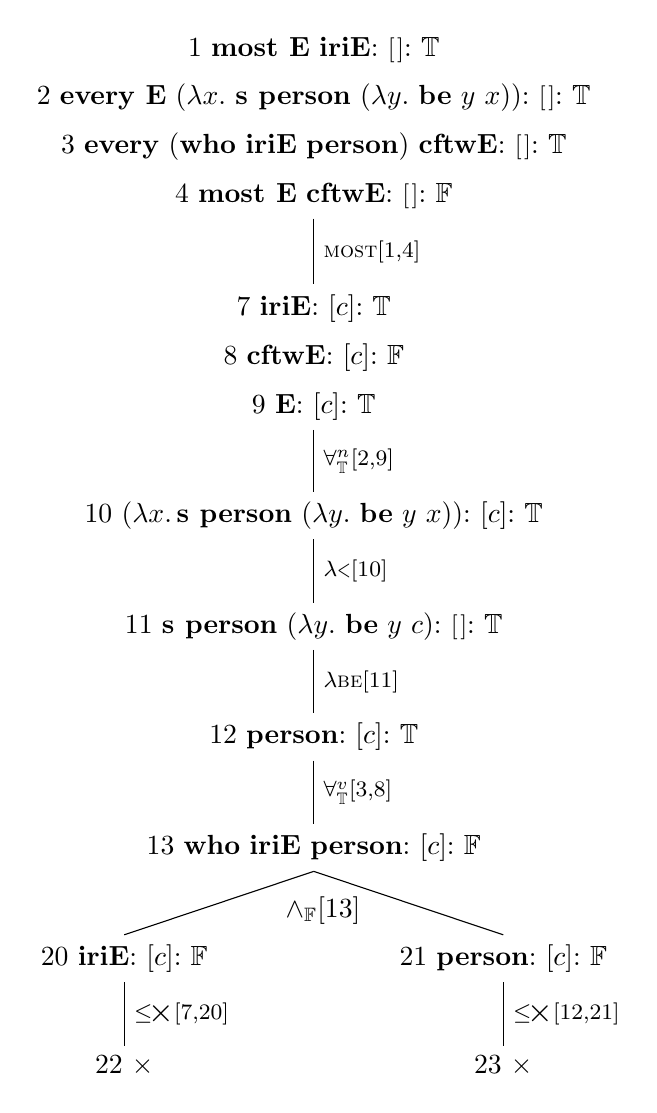
\begin{tikzpicture}[grow=down]
\tikzset{level distance = 40pt, sibling distance = 55pt}
\tikzset{every tree node/.style={align=center,anchor=north}}
\tikzset{level 1/.style={level distance=93pt}}	
\tikzset{level 2/.style={level distance=75pt}}	
\Tree
[.\node{\lab{1}~\synt{most E} \synt{iriE}:~$\elist$:~$\T$\\
\lab{2}~\toppad{5mm}\synt{every E} $(\lambda x.$~\synt{s person} $(\lambda y.$~\synt{be} $y$ $x$)):~$\elist$:~$\T$\\
\lab{3}~\toppad{5mm}\synt{every} (\synt{who} \synt{iriE} \synt{person}) \synt{cftwE}:~$\elist$:~$\T$\\
\lab{4}~\toppad{5mm}\synt{most E} \synt{cftwE}:~$\elist$:~$\F$};
\edge[right,font=\footnotesize] node{\ruleApp[1,4]{most}};
[.\node{\lab{7}~\synt{iriE}:~{[$c$]}:~$\T$\\
\lab{8}~\toppad{5mm}\synt{cftwE}:~{[$c$]}:~$\F$\\
\lab{9}~\toppad{5mm}\synt{E}:~{[$c$]}:~$\T$};
\edge[right,font=\footnotesize] node{\ruleApp[2,9]{$\forall^n_\T$}};
[.\node{\lab{10}~$(\lambda x.$\,\synt{s person} $(\lambda y.$~\synt{be} $y$ $x))$:~{[$c$]}:~$\T$};
\edge[right,font=\footnotesize] node{\ruleApp[10]{$\lambda \pull$}};
[.\node{\lab{11}~\synt{s person} $(\lambda y.$~\synt{be} $y$ $c$):~$\elist$:~$\T$};
\edge[right,font=\footnotesize] node{\ruleApp[11]{\rulen{$\lambda$be}}};
[.\node{\lab{12}~\synt{person}:~{[$c$]}:~$\T$};
\edge[right,font=\footnotesize] node{\ruleApp[3,8]{$\forall^v_\T$}};
[.\node[label={[label distance=2mm]-90:~~\ruleApp[13]{$\wedge_\F$}}]{\lab{13}~\synt{who} \synt{iriE} \synt{person}:~{[$c$]}:~$\F$};
	[.\node{\lab{20}~\synt{iriE}:~{[$c$]}:~$\F$};
	\edge[right,font=\footnotesize] node{\ruleApp[7,20]{\clrule}};
	 [.\node{\lab{22}~$\times$};]
	]
	[.\node{\lab{21}~\synt{person}:~{[$c$]}:~$\F$};
	\edge[right,font=\footnotesize] node{\ruleApp[12,21]{\clrule}};
	 [.\node{\lab{23}~$\times$};]
	]
]]]]]]
\end{tikzpicture}
}
\caption{The tableau proof, generated by LangPro, classifies Fr-26 as entailment. 
The abbreviations $\synt{cftwE}, \synt{iriE}$ and $\synt{E}$ stand for the LLFs of {\em can freely travel within Europe}, {\em is resident in Europe} and {\em European}, respectively.
The nodes that do not contribute to the closure of the tableau are omitted.
The proof also employs the admissible rules ($\forall^n_\T$) and ($\forall^v_\T$) from Section\,\ref{sec:efficient}.}
\label{fig:fracas-26}
\end{figure}
%{\em Most Europeans are resident in Europe. All Europeans are people. All people who are resident in Europe can travel freely within Europe $\Rightarrow$ Most Europeans can travel freely within Europe}.

 
 
FrSec-1 involves problems dedicated to the conservativity phenomenon \eqref{eq:conserv}.
Although we have not specially modeled the conservativity property of GQs in LangPro, it is able to solve all 16 poblems about conservativity except one.
The reason is that conservativity is underrepresented in FraCaS.
Namely, the problems cover conservativity in the form of \eqref{eq:there_conserv} instead of \eqref{eq:conserv} (see Fr-6).  
%
\begingroup
\setlength{\abovedisplayskip}{3mm}
\setlength{\belowdisplayskip}{3mm}
\setlength{\abovedisplayshortskip}{2mm}
\setlength{\belowdisplayshortskip}{2mm}
\begin{align}
Q~A~\text{are}~B \leftrightarrow & ~Q~A~\text{are}~A~\text{who are}~B \label{eq:conserv}
\\
Q~A~\text{are}~B \leftrightarrow & ~\text{There are}~Q~A~\text{who are}~B
\label{eq:there_conserv}
\end{align}
\endgroup
%
We capture \eqref{eq:there_conserv} with the help of the existing rules for GQs and (\rulen{thr}$\!\btimes$), from \cite{abzianidze:2015:LENLS}, which treats the expletive constructions, like {\em there is}, as a universal predicate, i.e., any entity not satisfying it leads to inconsistency ($\btimes$).  

  
%\addlater{Example proof for the expletive rule and quasy qonsevatiivity, most A are B cannot be done to most As are As whos are Bs}

\begin{center}
\nonBranchingRule[\rulen{thr}$\!\btimes$]
{$\synt{be}~c~\synt{there} : \elist : \F$}
{$\btimes$}
\end{center}

But these rules are not enough for solving Fr-44 because the monotonicity rules cannot lead to the solution when applied to the following nodes representing P1 and C of Fr-44, respectively.
%
\begingroup
\setlength{\abovedisplayskip}{3mm}
\setlength{\belowdisplayskip}{3mm}
\setlength{\abovedisplayshortskip}{2mm}
\setlength{\belowdisplayshortskip}{2mm}
\begin{align}
\synt{few}~ M~ (\synt{be}~ \synt{from}~ S) : \elist : \T
\label{nd:few1}\\
\synt{few}~ (\synt{from}~ P~ M)~ (\lambda x.\,\synt{be}~ x~ \synt{there}) : \elist : \F
\label{nd:few2}
\end{align}
\endgroup
%

To solve Fr-44, we introduce a new tableau rule (\rulen{thr\_pp}) which acts as a paraphrase rule.
After the rule is applied to \eqref{nd:few2}, (\rulen{mon}$\downarrow$) can be applied to the resulted node and \eqref{nd:few1} which contrasts {\em being from southern Europe} to {\em being from Portugal}. 

\begin{center}
\nonBranchingRule[\rulen{thr\_pp}]
{$Q~ (p_{\np,\nou,\nou} A~ N)(\lambda x.\, \synt{be}~x~\synt{there}) : \elist : \X$}
{$Q~ N~ (\synt{be}~(p~A)) : \elist : \X$}
\end{center}

FrSec-2 covers the problems concerning plurals. 
Usually the phrases like bare plurals, definite plurals and definite descriptions (e.g., {\em the dog}) do not get special treatment in wide-coverage semantic processing and by default are treated as indefinites.
Since we want to take advantage of the expressive power of the logic and its proof system, we decide to separately model these phrases.
We treat bare plurals and definite plurals as GQs of the form $\synt{s}_{\nou,\vp,\sen}\,N_\nou$, where $\synt{s}$ stands for the plural morpheme.
%it is considered to be upward monotone in both argument positions,
%therefore licensing the entailment $\synt{s~dog~run} \to \synt{s~animal~move}$.  
The quantifier $\synt{s}$ can be ambiguous in LLFs due to the ambiguity related to the plurals: they can be understood as {\em more than one}, {\em universal} or {\em quasi-universal} (i.e. {\em almost every}).
Since most of the problems in FraCaS favor the latter reading, we model $\synt{s}$ as a quasi-universal quantifier.
We introduce the following lexical knowledge, $\synt{s} \leq \synt{a}$ and $\synt{s} \leq \synt{most}$, in the KB and allow the existential quantification rules (e.g., $\exists_\T$) to apply the plural terms $\synt{s}\,N$.     
With this treatment, for instance, the prover is able to prove the entailment in Fr-100.



We model the definite descriptions as generalized quantifiers of the form $\synt{the}\,N$, where the rules make $\synt{the}$ act as the universal and existential quantifiers when marked with $\T$ and as the existential quantifier  in case of $\F$.
Put differently, ($\forall_\T$), ($\exists_\T$) and ($\exists_\F$) allow the quantifier in their antecedent nodes to match $\synt{the}$.

\begin{center}
\parbox{46mm}{
%forall T
\BranchingRule[$\forall_\T$\\$g \in \{\synt{every},\synt{the}\}$ and $c_e$ is old]
{$g_\qu~N~V : \elist : \T$}
{$N : [c_e] : \F$}
{$V : [c_e] : \T$}
\\[2mm]
%exists F
\BranchingRule[$\exists_\F$\\$g \in \{\synt{a},\synt{the}\}$ and $c_e$ is old]
{$g_\qu~N~V : \elist : \F$}
{$N : [c_e] : \F$}
{$V : [c_e] : \F$}
}
\nonBranchingRule[$\exists_\T$\\$g \in \{\synt{a},\synt{s},\synt{the}\}$\\and $c_e$ is fresh]
{$g_\qu~N~V : \elist : \T$}
{$N : [c_e] : \T$\\$V : [c_e] : \T$}
\end{center}
%
This choice guarantees that, for example, {\em the demonstration} in the premises of Fr-99 co-refer and allow the proof for entailment.
This approach also maintains the link if there are different surface forms co-referring, e.g., {\em the demonstration} and {\em the presentation}, in contrast to the approach in \newcite{abzianidze:2015:EMNLP}.  


FrSec-2 also involves several problems with contrasting cardinal phrases like $\synt{exactly}~n$ and $m$, where $n < m$ (see Fr-85).
We account for these problems with the closure rule ($\btimes$\,\rulen{exct}), where the type $\qu$, the predicate ${\tt greater}/2$ and the domain for $E$ act as constraints.

\begin{center}
\nonBranchingRule[$\btimes$\,\rulen{exct}]
{$E_{\qu,\qu} N_\qu : [\vv{C}] : \T$\\
 $M_\qu   : [\vv{C}] : \T$}
{$\btimes$}
~
\parbox{35mm}{such that\\
$E \in \{\synt{just}, \synt{exactly}\}$
\\and ${\tt greater}(M,N)$
}
\end{center}


FrSec-5 contains RTE problems pertaining to various types of adjective.   
First-order logic has problems with modeling {\em subsective} or {\em privative} adjectives \cite{Kamp-partee:1995}, but they are naturally modeled with higher-order terms.
A subsective term, e.g., $\synt{ small}_{\nou,\nou}$, is a relation over a {\em comparison class} and an entity, e.g., $\synt{small}_{\nou,\nou}~\synt{animal}_\nou\,c_e$ is of type $t$ as $\nou$ is a subtype of $et$ according to the extended type theory \cite{abzianidze:2015:LENLS}.
The rule ($\subseteq$) in Figure~\ref{fig:intro_rules} accounts for the subsective property.
With the help of it, the prover correctly identifies Fr-211 as contradiction (see Figure~\ref{fig:dumbo}).
%The tableau proof closes as the nodes \lab{10} and \lab{11} are found inconsistent with the help of the ($\btimes|$) rule.
In case of the standard first-order {\em intersective} analysis, the premises of Fr-211 would be translated as:
\\[2mm]
$\semt{small}(\semt{dumbo}) \wedge \semt{elephant}(\semt{dumbo}) \wedge\\ \forall x\big(\semt{elephant}(x) \to (\semt{large}(x) \wedge \semt{animal}(x))\big)$
\\[2mm]
which is a contradiction given that $\semt{small}$ and $\semt{large}$ are contradictory predicates.
Therefore, due to the {\em principle of explosion} everything, including the conclusion and its negation, would be entailed from the premises. 



\begin{figure}[t]
\hspace{-4mm}
\scalebox{.8}{
\begin{forest}
for tree={align=center, parent anchor=south, child anchor=north, l sep=7mm}
[{\lab{1}~  
  $\synt{every} ~ \synt{elephant} ~ (\lambda x.\,\synt{s} ~ (\synt{large} ~ \synt{animal}) ~ (\lambda y\,\synt{be} ~ y ~ x)) : \elist : \T$}\\
 {\lab{2}~\toppad{5mm}  
   $\synt{a} ~ (\synt{small} ~ \synt{elephant}) ~ (\lambda x.\,\synt{be} ~ x ~ \synt{dumbo}) : \elist : \T$}\\
 {\lab{3}~\toppad{5mm}  
    $\synt{a} ~ (\synt{small} ~ \synt{animal}) ~ (\lambda x.\,\synt{be} ~ x ~ \synt{dumbo}) : \elist : \T$}
   [{\lab{4}~ 
     $\synt{small} ~ \synt{animal} : [\synt{dumbo}] : \T$}, edge label={node[left,midway,font=\footnotesize]{\ruleApp[3]{$\lambda$be}}}
    [{\lab{5}~  
      $\synt{small} ~ \synt{elephant} : [\synt{dumbo}] : \T$}, edge label={node[left,midway,font=\footnotesize]{\ruleApp[2]{$\lambda$be}}}
     [{\lab{6}~ 
       $\synt{elephant} : [\synt{dumbo}] : \T$}, edge label={node[left,midway,font=\footnotesize]{\ruleApp[5]{$\subseteq$}}}
      [{\lab{7}~ 
        $\lambda x.\,\synt{s} ~ (\synt{large} ~ \synt{animal}) ~ (\lambda y.\,\synt{be} ~ y ~ x) : [\synt{dumbo}] : \T$}, edge label={node[left,midway,font=\footnotesize]{\ruleApp[1,6]{$\forall_\T^n$}}}
       [{\lab{8}~  
         $\synt{s} ~ (\synt{large} ~ \synt{animal}) ~ (\lambda y.\,\synt{be} ~ y ~ \synt{dumbo}) : \elist : \T$}, edge label={node[left,midway,font=\footnotesize]{\ruleApp[7]{$\lambda\pull$}}}
        [{\lab{9}~  
          $\synt{large} ~ \synt{animal} : [\synt{dumbo}] : \T$}, edge label={node[left,midway,font=\footnotesize]{\ruleApp[8]{$\lambda$be}}}
         [{\lab{10}~  
          $\synt{small} : [\synt{animal},\synt{dumbo}] : \T$}\\
          {\lab{11}~\toppad{5mm}  
          $\synt{large}  : [\synt{animal},\synt{dumbo}] : \T$}, edge label={node[left,midway,font=\footnotesize]{\ruleApp[4,9]{$\push$}}} 
          [{\lab{12}~$\btimes$}, edge label={node[left,midway,font=\footnotesize]{\ruleApp[10,11]{$\btimes \mid$\,}}}
          ]
         ] 
        ]
       ]
      ]
     ]
    ]
   ]
]
\end{forest} 
}
\caption{The closed tableau by LangPro proves Fr-211 as contradiction.
%The rule (\rulen{$\lambda$be}) significantly decreases the size of the tableau.
}
\label{fig:dumbo}
\end{figure}


FrSec-9, about attitudes, is the last section we explore.
Though the tableau system of \cite{muskens:10} employs intensional types, LangPro only uses extensional types due to simplicity of the system and the paucity of intensionality in RTE problems.
Despite the fact, with the proof-theoretic approach and extensional types, we can still account for a certain type of reasoning on attitude verbs by modeling entailment properties of the verbs in the style of \newcite{nairn:2006} and \newcite{karttunen:2012:STARSEM-SEMEVAL}.
For example, {\em know} has (+$/$+) property meaning that when it occurs in a positive embedding context, it entails its sentential complement with a positive polarity.
Similarly, {\em manage to} is (+$/$+) and (-$/$-) because {\em John managed to run} entails {\em John run} and {\em John did not manage to run} entails {\em John did not run}.
% while {\em believe} has none of the four entailment properties.   
We accommodate the entailment properties in the tableau system in a straightforward way, e.g., terms with (+$/$+) property, like $\synt{know}$ and $\synt{manage}$, are modeled via the rule (+$/$+) where $?p$ is an optional prepositional or particle term.
The rest of the three entailment properties for attitude verbs are captured in the similar way.     

\begin{center}
\nonBranchingRule[~+$/$+]
{$h^{\text{++}}_{\alpha,\vp} (?p_{\alpha,\alpha} ~ V_\alpha) : [d] : \T$}
{$V_\alpha : [\vv{E}] : \T$}
\\such that if $\alpha = \vp$, then $\vv{E} = d$; 
\\otherwise $\alpha = \sen$ and $\vv{E}$ is empty 
\end{center}  

We also associate the entailment properties with the phrases {\em it is true that} and {\em it is false that} and model them via the corresponding tableau rules.
%In order to enable substitution 

Our account for intensionality with the extensional types represents a syntactic approach rather than semantic.
From the semantics perspective, the extensional types license John knowing all true statement if he knows at least one of them.
But using the proof system, a syntactic machinery, we avoid such unwanted entailments with the absence of rules.
In future, we could incorporate intensional types in LangPro if there is representative RTE data for the intensionality phenomenon.  


The rest of the FraCaS sections were skipped during the adaptation phase for several reasons.
FrSec-3 and FrSec-4 are about anaphora and ellipsis respectively.
We omitted these sections as recently pronoun resolution is not modeled in the natural tableau and almost all sentences involving ellipsis are wrongly analyzed by the CCG parsers.
In the current settings of the natural tableau, we treat auxiliaries as vacuous, due to this reason LangPro cannot properly account for the problems in FrSec-8 as most of them concern the aspect of verbs.
FrSec-6 and FrSec-7 consists of problems with comparatives and temporal reference respectively.
To account the latter phenomena, the LLFs of certain constructions needs to be specified further (e.g., for comparative phrases) and additional tableau rules must be introduced that model {\em calculations} on time and degrees.   


%For comparatives, we need to decide how they are modeled in LLFs and to add new rules that account for their semantic properties, e.g., transitivity, while for temporal reference, we can introduce event entities that will be related to time 



\section{Efficient theorem proving}
\label{sec:efficient}

%On the other hand, the choices in rule applications increase with the increased number of premises.
%This decreases the chance of finding a sequence of rule applications that promptly leads to the branch closure, hence to short proofs.    

Efficiency in theorem proving is crucial as we do not have infinite time to wait for provers to terminate and return an answer.
Smaller tableau proofs are also easy for verifying and debugging.
The section discusses the challenges for efficient theorem proving induced by the FraCaS problems and introduces new rules that bring efficiency to some extent.
 
The inventory of rules is a main component of a tableau method.
Usually tableau rules are such inference rules that their consequent expressions are not larger than the antecedent expressions and are built up from sub-parts of the antecedent expressions.
The natural tableau rules also satisfy these properties which contribute to the termination of tableau development.
But there is still a big chance that a tableau does not terminate or gets unnecessarily large.
The reasons for this is a combination of branching rules, $\delta$-rules (introducing fresh entity terms), $\gamma$-rules (triggered for each entity term), and non-equivalent rules (the antecedents of which must be accessible by other rules too).%   
%
\footnote{For instance, (\rulen{mon}$\uparrow$) and (\rulen{mon}$\downarrow$) in Figure\,\ref{fig:intro_rules} are both branching and $\delta$.
They are also non-equivalent since their consequents are semantically weaker than their antecedents;
this requires that after their application, the antecedent nodes are still reusable for further rule applications. 
On the other hand, ($\forall_\T$) is non-equivalent and $\gamma$;
for instance, for any entity term $c_e$, it is applicable to $\synt{every}~\synt{dog}~\synt{bark}\Co\elist\Co\T$ and asserts that either $c$ is not $\synt{dog}$ or $c$ does $\synt{bark}$.  
}
Efficeint theorem proving with LangPro becomes more challenging with multi-premised problems and monotonic GQs.
More nodes in a tableau give rise to more choice points in rule applications and monotonic GQs are usually available for both monotonic and standard semantic rules.


To encourage short tableau proofs, we introduce eight {\em admissible} rules --- the rules that are redundant from completeness point of view but represent {\em smart} shortcuts of several rule applications.%
%
\footnote{In other words, if a closed tableau makes use of an admissible rule, the tableau can still be closed with a different rule application strategy that ignores the admissible rule.
}  
Half of the rules for the existential (e.g., {\em a} and {\em the}) and universal (e.g., {\em every}, {\em no} and {\em the}) quantifiers are $\gamma$-rules.%
%
\footnote{Remember from Section\,\ref{sec:model} that $the$ is treated like the universal and existential quantifiers in certain cases. 
}
To make application of these rules more efficient, we introduce two admissible rules for each of the $\gamma$-rules. 
For instance, ($\forall^{n}_\T$) and ($\forall^{v}_\T$) are admissible rules which represent the efficient but incomplete versions of ($\forall_\T$): 

\begin{center}
\nonBranchingRule[$\forall^n_\T$]
%\parbox{45mm}{where $q \in \{\synt{every},\synt{the}\}$,
%\\$(A, B) = (N,V)$ if $\X=\T$\\
%otherwise $(A, B) = (V,N)$}]
{$q~N~V : \elist : \T$\\
 $N : [c] : \T$
}
{$V : [c] : \T$}
~
\nonBranchingRule[$\forall^v_\T$]
%\parbox{45mm}{where ,
%\\$(A, B) = (N,V)$ if $\X=\T$\\
%otherwise $(A, B) = (V,N)$}]
{$q~N~V : \elist : \T$\\
 $V : [c] : \F$
}
{$N : [c] : \F$}
\\
where $q \in \{\synt{every},\synt{the}\}$
\end{center}
%
Their efficiency is due to choosing a relevant entity $c_e$, rather than any entity like ($\forall_\T$) does: ($\forall^{n}_\T$) chooses the entity that satisfies the noun term while ($\forall^{v}_\T$) picks the one not satisfying the verb term. 
Moreover, the admissible rules are not branching unlike their $\gamma$ counterparts.
Other four admissible rules account for {\em a} and {\em the} in a false context and {\em no} in a true context in the similar way. 


The monotonicity rules, (\rulen{mon$\uparrow$}) and (\rulen{mon$\downarrow$}), are inefficient as they are branching $\delta$-rules.
On the other hand, the rules for GQs are also inefficient for being a $\gamma$ or $\delta$-rule.
Both types of rules are often applicable to the same GQs, e.g., {\em every} and {\em a}, as most of GQs have monotonicity properties.
Instead of triggering these two types of rules separately, we introduce two admissible rules, (\rulen{$\exists$fun$\uparrow$}) and (\rulen{$\emptyset$fun$\downarrow$}), which trigger them in tandem:%
%
%\footnote{Notice similarities and differences between (\rulen{$\exists$fun$\uparrow$}) and (\rulen{most}).}


\begin{center}
\tabuc{
\nonBranchingRule[\rulen{$\exists$fun$\uparrow$}]
{$g_\qu \, N \, A : \elist : \T$ \lab{1} 
\\$g_\qu \, N \, B : \elist : \F$ \lab{2}}
{$A: [c_e] :\T$ \lab{3} \\ $B: [c_e]: \F$ \lab{4} \\ $N: [c_e]: \T$ \lab{5}}
\\
$g \in \{\synt{a}, \synt{s}, \synt{many}, \synt{every}\}$
}
\tabuc{
\nonBranchingRule[\rulen{$\emptyset$fun$\downarrow$}]
{$h_\qu \, N \, A : \elist : \F$ 
\\$h_\qu \, N \, B : \elist : \T$}
{$A: [c_e] :\T$ \\ $B: [c_e]: \F$ \\ $N: [c_e]: \T$}
\\
$h \in \{\synt{no}, \synt{few}\}$
}
\end{center}  
%
For instance, if $g = \synt{every}$, a single application of (\rulen{$\exists$fun$\uparrow$}) already yields the fine-grained semantics: there is $c_e$ that is $A$ and $N$ but not $B$.
If the nodes were processed by the rules for $\synt{every}$, ($\forall_\F$) would first entail \lab{4} and \lab{5} from \lab{2} and then ($\forall_\T$) or ($\forall_\T^n$) would introduce \lab{3} from \lab{1}.
(\rulen{$\exists$fun$\uparrow$}) also represents a more specific version of the admissible rule (\rulen{fun$\uparrow$}) of \newcite{abzianidze:2015:EMNLP}, which itself is an efficient and partial version of (\rulen{mon}$\uparrow$).  

(\rulen{$\exists$fun$\uparrow$}) and (\rulen{$\emptyset$fun$\downarrow$}) not only represent admissible rules but they also model semantics of {\em few} and {\em many} not captured by the monotonicity rules.
For instance, if $\synt{few}\,\synt{dog}\,\synt{bark}\Co\elist\Co\F$ and $\synt{few}\,\synt{dog}\,\synt{bite}\Co\elist\Co\T$, then a set of entities that are $\synt{dog}$ and $\synt{bark}$, denoted by $\sem{\synt{dog}} \cap \sem{\synt{bark}}$, is strictly larger than $\sem{\synt{dog}} \cap \sem{\synt{bite}}$ (despite the absolute or relative readings of {\em few}).
Due to this set relation, there is an entity in $\sem{\synt{dog}} \cap \sem{\synt{bark}}$ and not in $\sem{\synt{bite}}$.
Therefore, we get the inference encoded in (\rulen{$\emptyset$fun$\downarrow$}).
Similarly, it can be shown that {\em many} satisfies the inference in (\rulen{$\exists$fun$\uparrow$}).




%It is well known that the equality is a source of inefficiency in the theorem proving \cite{Fitting:1990}.
%In order to avoid modeling the copula as the equality relation, we introduce the rule (\rulen{$\lambda$be}), in Figure~\ref{fig:rules}, which is useful when analyzing the LLFs of the phrases like {\em all dogs are animals} or {\em each dog is an animal}.
%With the help of the rule, there is no need to introduce the entity for the object NP, e.g. {\em animals} or {\em an animal}, and equate it with the entity satisfying the subject noun.  
%Instead, the rule assigns the object noun as a property to the entity that satisfies the subject noun.


%The other admissible rules are the efficient versions of ({\sc mon$\uparrow$}) and ({\sc mon$\downarrow$}) corresponding the cases when the antecedent nodes share the functors ($G=H$) or the arguments ($A=B$). 
%The short tableau proof of a complex entailment problem in Figure\,\ref{fig:fracas-26} demonstrates efficiency of the admissible rules ($\forall_\T^c$) and (\rulen{$\exists$fun$\uparrow$}).


 

\begin{table}[t]
\hspace*{-3mm}
\scalebox{.86}{
\begin{tabular}{@{}c@{\,}|l@{}}\hline
ID  & \hspace{10mm} FraCaS entailment problem
\\\hline%--------------------------------------------
%\tabuc[t]{58\\unk} & 
%\toppad{4mm}\parbox[t]{85mm}{
%{\bf P}: Most Europeans who are resident in Europe can travel freely within Europe.\\ 
%{\bf C}: Most Europeans can travel freely within Europe.
%}\\\hline%--------------------------------------------
\tabuc[t]{64\\unk} & 
\toppad{4mm}\parbox[t]{83mm}{
{\bf P}: At most ten female commissioners spend time at home.\\
{\bf C}: At most ten commissioners spend time at home.
}\\\hline%----------------------------------------
\tabuc[t]{88\\unk} & 
\toppad{4mm}\parbox[t]{83mm}{
{\bf P}: Every representative and client was at the meeting.\\ 
{\bf C}: Every representative was at the meeting.
}\\\hline%--------------------------------------------
\tabuc[t]{109\\no} & 
\toppad{4mm}\parbox[t]{83mm}{
{\bf P}: Just one accountant attended the meeting.\\ 
{\bf C}: Some accountants attended the meeting.
}\\\hline%--------------------------------------------
\tabuc[t]{215\\unk} & 
\toppad{4mm}\parbox[t]{83mm}{
{\bf P1}: All legal authorities are law lecturers.\\
{\bf P2}: All law lecturers are legal authorities.\\
{\bf C}: All competent legal authorities are competent law lecturers.
}\\
\end{tabular}
}
\caption{Problems with false proofs}
\label{tab:analysis_probs}
\end{table}






%██████████████████ Evaluation ██████████████████████
\section{Evaluation}
\label{sec:eval}

After adapting the prover to the FraCaS sections for GQs, plurals, adjectives and attitudes, we evaluate it on the relevant sections and analyze the performance. Obtained results are compared to related RTE systems. 


We run two version of the prover, ccLangPro and easyLangPro, that employ CCG derivations produced by \candc{} and \easyccg{} respectively.
In order to abstract from the parser errors to some extent, the answers from both provers are aggregated in LangPro: a proof is found iff one of the parser-specific provers finds a proof.
The evaluation results of the three versions of LangPro on the relevant FraCaS sections are presented in Table\,\ref{tab:matrix} along with the confusion matrix for LangPro.





The results show that LangPro performs slightly better with \candc{} compared to \easyccg{}. 
This is due to \llfgen{} which is mostly tuned on the \candc{} derivations.
Despite this bias, easyLangPro proves 8 problems that were not proved by ccLangPro.
In case of half of these problems, \candc{} failed to return derivations for some of the sentences while in another half of the problems the errors in \candc{} derivations were crucial, e.g., in the conclusion of Fr-44 {\em committee members} was not analyzed as a constituent. 
On the other hand, ccLangPro proves 10 problems unsolved by easyLangPro, e.g., Fr-6 was not proved because \easyccg{} analyzes {\em really} as a modifier of {\em are} in the conclusion, or even more unfortunate, the morphological analyzer of \easyccg{} cannot get the lemma of {\em clients} correctly in Fr-99 and as a result the prover cannot relate $\synt{clients}$ to $\synt{client}$. 



\begin{table}[t]
\scalebox{.95}{
\begin{tabular}{|@{\,}l@{\,}|@{\,}c@{\,}|@{\,}c@{\,}|@{\,}c@{\,}|@{\,}c@{\,}|}
\hline
Meas\% 	& ccLP 	& eLP 	& \bf LP\\\hline\hline
Prec 	& \bf94	& 93 	&\bf 94\\
Rec 	& 73 	& 71 	&\bf 81\\
Acc 	& 80 	& 79 	&\bf 85\\\hline
\end{tabular} 
~
\begin{tabular}{|@{\,}l@{\,}||@{\,}c@{\,}|@{\,}c@{\,}|@{\,}c@{\,}|}
\hline
Gold$\backslash$\bf LP 	&{\sc yes} 	&{\sc no} 	&{\sc unk} \\\hline\hline
{\sc yes} 			& \bf60  	& 0 		& 14 \\
{\sc no}  			& 1			& {\bf 14} 	& 2 \\
{\sc unk} 			& 4 		& 0 		& \bf47 \\\hline
\end{tabular} 
}
\caption[]{Measures of ccLangPro (ccLP), easyLangPro (eLP) and LangPro (LP) on FraCaS sections 1, 2, 5, 9 and the confusion matrix for LP.}
\label{tab:matrix}
\end{table}



\begin{table*}
\centering
\scalebox{.80}{
%\begin{small}
\begin{tabular}{|l@{~}r@{\,}| %2
|@{}c@{\,}|@{\,}c@{\,}|@{\,}c@{\,}|@{\,}c@{\,}|@{\,}c@{\,}|@{\,}c@{\,}|@{\,}c@{\,}| % 7
|@{}c@{\,}|@{\,}c@{\,}|@{\,}c@{\,}|@{\,}c@{\,}|@{\,}c@{\,}|  % 5
|@{}c@{\,}|@{\,}c@{\,}|@{\,}c@{\,}|@{\,}c@{\,}|@{\,}c@{\,}|} % 5
\hline
\multicolumn{2}{|@{}c@{}||}{\multirow{2}{*}{Sec (Sing/All)}} & 
\multicolumn{7}{@{}c@{}||}{Single-premised (Acc \%)} & 
\multicolumn{5}{@{}c@{}||}{~Multi-premised (Acc \%)~} &
\multicolumn{5}{@{}c@{}|}{Overall (Acc \%)}
\\\cline{3-19}\toppad{5mm}
&      
&\,BL &NL07,08 &LS P/G &NLI &T14a,b &M15 &\bf LP &\,BL &LS P/G &T14a,b &M15 &\bf LP &\,BL &LS P/G &T14a,b &M15 &\bf LP\\\hline
\toppad{5mm}1 GQs &(44/74)
&45 &84~~\bf98 &70~~89 &95 &80~~93 &82     & 93 &57 &50~~80 &80~~\bf97 &73   &93 &50  &62~~85 &80~~\bf95 &78 &93
\\
2 Plur &(24/33)
&58 &\sout{42}~~\bf75 & -  &\sout{38}   &-  &67 &\bf75  &67 &-  &-   &67   &67 &61  &- &- &67 &\bf73
\\
5 Adj &(15/22)
&40 &60~~80 & -  &\bf87   &-  &\bf87 &\bf87 &43  &-    &-   &29 &43 &41 &- &- &68 &\bf73
\\   
9 Att & (9/13)
&67 &\sout{56}~~89 & - &\sout{22} &- &78 &\bf100 &50 &- &- &\bf75 &\bf75 &62 &- &- &77 &\bf92 
\\\hline
\toppad{5mm}1,2,5,9 & (92/142) 
&50 &\,\,-\,\,~~\bf88 &- &- &- &78 &\bf88 &56 &- &- &66 &\bf80 &52 &- &- &74 &\bf85
\\\hline
\end{tabular} 
%\end{small}
}
\caption[]{Comparison of RTE systems tested on FraCaS: NL07 \cite{MacCartney:07}, NL08 \cite{MacCartney:08}, LS \cite{lewis-steedman:13} with Parser and Gold syntax, NLI \cite{naturalli}, T14a \cite{tian-miyao-matsuzaki:2014:P14-1}, T14b \cite{Dong-EtAl:2014:PACLIC} and M15 \cite{mineshima-EtAl:2015:EMNLP}.
BL is a majority ({\em yes}) baseline.
Results for non-applicable sections are strikeout.}
\label{tab:comparison}
\end{table*}


The precision of LangPro is high due to its sound inference rules.
Fr-109 in Table\,\ref{tab:analysis_probs} was the only case when entailment and contradiction were confused: plurals are not modeled as strictly more than one.%
%
\footnote{Moreover, Fr-109 is identical to Fr-107 which has {\em yes} as a gold answer.
Another inconsistency in gold answers of Fr-87 and Fr-88 (due to the ambiguous premise) is a reason for a false proof.
While Fr-87 was correctly proved by the prover, obviously Fr-88 was misclassified automatically.
}
The false proves are mostly due to a lack of knowledge about adjectives. 
LangPro does not know a default comparison class for {\em clever}, e.g., {\em clever person}$\to${\em clever} but {\em clever politician}$\not\to${\em clever}).
Fr-215 was proved as entailment because we have not modeled intensionality of adjectives. 
Since \easyccg{} was barely used during adaptation (except changing most of NP modifiers into noun modifiers), it analyzed {\em at most} in Fr-64 as a sentential modifier which was not modeled as downward monotone in the signature.
Hence, by default, it was considered as upward monotone leading to the proof for entailment.   






There are several reasons behind the problems that were not proved by the prover.
Several problems for adjectives were not proved as they contained comparative constructions, not covered by the rules.
Some problems assume the universal reading of plurals.
A couple of problems involving {\em at most} were not solved as the parsers often analyze the phrase in a wrong way.%    
% 
\footnote{Tableau proofs of the FraCaS problems are available at: \url{http://lanthanum.uvt.nl/langpro/fracas}
} 
%In most of the cases, the parsers are responsible for the failure in the proof search.
%For instance, the parsers were not able to return derivations for around 5 sentences while in several obtained derivations there were errors crucial for the proofs.
%The errors from the parsers are not surprising if we take into account that the sentences they are trained on are much more longer than what we find in FraCaS.%

We also check the FraCaS sections how representative they are for higher-order GQs (HOGQs).
After replacing all occurrences of $\synt{most}$, $\synt{several}$, $\synt{many}$, $\synt{s}$ and $\synt{the}$ with the indefinite $\synt{a}$ in LLFs, LangPro$^{\textsc{--hogq}}$ (without the HOGQs) achieves an overall accuracy of 81\% over FrSec-1,2,5,9.
Compared to LangPro only 6 problems, including Fr-56,\,99, were misclassified while Fr-26,\,100 were solved. 
This shows that the dataset is not representative enough for HOGQs. 


%To measure the impact of admissible rules, we tested the prover without the admissible rules on Sections 1, 2, 5 and 9.
%The results showed decrease in accuracy by 10\% (around 12 problems).
%Most vital admissible rule happens to be ($\forall_\T^c$).
%This is explained by the frequent involvement of the universal quantifiers in multi-premised problems. 
%
%



In Table\,\ref{tab:comparison}, the current results are compared to the RTE systems that have been tested on the single or multi-premised FraCaS problems.%
%
\footnote{
Since the FraCaS data is small and usually the problems are seen during the system development, the comparison should be understood in terms of an expressive power of a system and the underlying theory.
}
According to the table, the current work shows that the natural tableau system and LangPro are successful in deep reasoning over multiple premises. 

The natural logic approach in \newcite{MacCartney:08} and \newcite{naturalli}  models monotonicity reasoning with the exclusion relation in terms of the string edit operations over phrases.
Since the approach heavily hinges on a sequence of edits that relates a premise to a conclusion, it cannot process multi-premised problems properly.
\newcite{lewis-steedman:13} and \newcite{mineshima-EtAl:2015:EMNLP} both base on first-order logic representations.
While \newcite{lewis-steedman:13} employs distributional relation clustering to model the semantics of content words, \newcite{mineshima-EtAl:2015:EMNLP} extends first-order logic with several higher-order terms (e.g., for {\em most, believe, manage}) and augments first-order inference of Coq with additional inference rules for the higher-order terms. 
\newcite{tian-miyao-matsuzaki:2014:P14-1} and \newcite{Dong-EtAl:2014:PACLIC} build an inference engine that reasons over abstract denotations, formulas of relational algebra or a sort of description logic, obtained from Dependency-based Compositional Semantic trees \cite{liang11dcs}.
Our system and approach differ from the above mentioned ones in its unique combination of expressiveness of high-order logic, {\em naturalness} of logical forms (making them easily obtainable) and flexibility of a semantic tableau method.
All these allow to model surface and deep semantic reasoning successfully in a single system.       




%██████████████████ Future Work █████████████████
\section{Future work}
\label{FW}

We have modeled several semantic phenomena in the natural tableau theorem prover and obtained high results on the relevant FraCaS sections.
Concerning the FraCaS dataset, in future work we plan to account for the comparatives and temporal reference in the natural tableau.
After showing that the natural tableau can successfully model deep reasoning (e.g., the FraCaS problems) and (relatively) wide-coverage and surface reasoning (e.g., the \sick{} dataset), we see the RTE datasets, like RTE-1 \cite{Dagan:2005} and SNLI \cite{bowman-EtAl:2015:EMNLP}, involving texts obtained from newswire or crowd-scouring as a next step for developing the theory and the theorem prover.        
 




\section*{Acknowledgments}

The author thanks the anonymous reviewers for their valuable comments and feedback.
The research is a part of the project ``Towards Logics that Model Natural Reasoning" supported by the NWO grant (project number 360-80-050).
 


\bibliography{myACLref}
%\bibliography{acl2016}
\bibliographystyle{acl2016}




\end{document}
